\chapter{Fejlesztői dokumentáció}
\label{ch:impl}

Ebben a fejezetben részletesen ismertetem az elkészített programkönyvtár működését, felépítését és a fejlesztési folyamat közben hozott döntések és javítások jelentősségét. Bemutatom a szoftver tesztelésének lépéseit és a vizualizációs integrációt is. Kitérek még az útvonaltervező szoftver részleteire és elméleti hátterére is, amihez az általam kidolgozott modul is tartozik.

\section{Elméleti háttér}

\subsection{A jármű kinematikai modellje}

Mielőtt a használt A* algoritmus útvonalat tudna keresni, fontos megismerni az algoritmus álltal használt gráfcsúcsok adatainak elméleti hátterét. Ezt egy kinematikai egypályás modellel (később STM) reprezentáljuk, aminek a lényege, hogy lefedje a jármű $x$ és $y$ koordinátáját a koordinátarendszerben, valamint a jármű orientációját ($\theta$). Ezek segítségével kapjuk a következő modellt \cite{kug_obp}:
\begin{align}
    x' &=v\cos(\theta) \\
    y' &=v\sin(\theta) \\
    \theta' &=\frac{v}{L}\tan(\delta)
\end{align}

Az első két egyenlet a jármű sebességét ($v$) bontja $x$ és $y$ irányú komponensekre, a harmadik egynelet pedig a jármű orientációjának változását írja le a kormányzott kerekek állásának szöge ($\delta$) és a tengelyhossz ($L$) függvényében. Mind $v$ és $\delta$ bemeneti adatok, csak $L$ paraméter az egyenletrendszerben. \\
Az előző egyenletrendszerben viszont nem szerepelt korlátozás a kormányzott kerekek szögének változására, tehát matematikailag lehetséges lenne az ugrásszerű változás is. Hogy ezt elkerüljük, a kerekek szögét ($\delta$) is bevezetjük, mint állapot és helyette a kerékállások változásának a szögsebessége ($v_\delta$) lesz a második bemeneti adat. Tehát a végső modell:
\begin{align}
    x' &=v\cos(\theta) \\
    y' &=v\sin(\theta) \\
    \theta' &=\frac{v}{L}\tan(\delta) \\
    \delta' &=v_\delta
\end{align}

\begin{figure}[H]
	\centering
	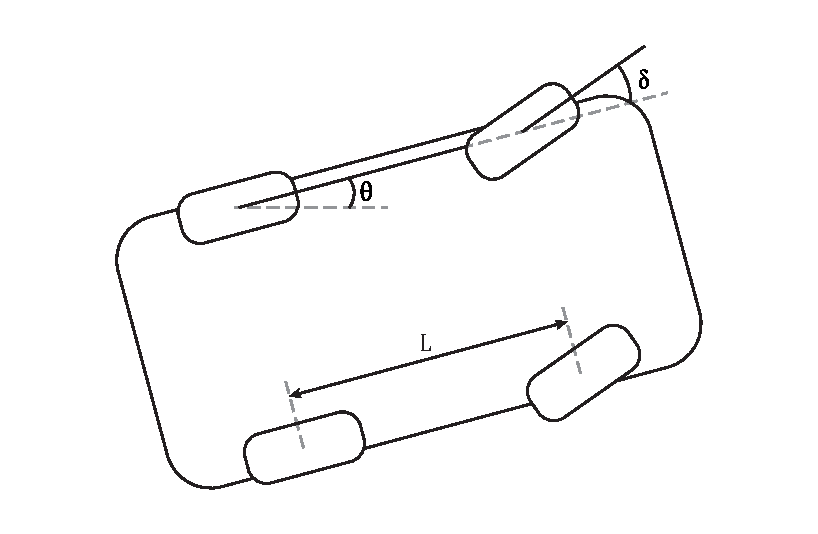
\includegraphics[width=300px]{stm_graphic}
	\caption{Az STM geometriai vizualizációja}
	\label{fig:STMdrawing}
\end{figure}

Az $[x, y, \theta, \delta]^T$ négyest a forráskódban a
{\fontfamily{cmtt}\selectfont rbp::pp::common::CPosture} osztály reprezentálja, amely \az\told{\ref{src:CPostureClass}}+as{} kódrészletben látható.

\begin{note}
A (\ref{src:CPostureClass}) osztályhoz hasonlóan léteznek a benne szereplő {\fontfamily{cmtt}\selectfont rbp::pp::common::CPose} ($[x, y, \theta]^T$) és az azon belüli {\fontfamily{cmtt}\selectfont rbp::pp::common::CPosition} ($[x, y]^T$) osztályok is. A \emph{getter} és \emph{setter} függvények helymegtakarítás miatt nincsenek megjelenítve, intuitívan állítható és lekérdezhető az $x, y, \theta, \delta$ paraméter ($x, y, \theta$ egyben is mint {\fontfamily{cmtt}\selectfont CPose} és $x, y$ mint {\fontfamily{cmtt}\selectfont CPosition}).
\end{note}
\clearpage

\lstset{caption={A CPosture osztály kivonata}, label=src:CPostureClass}
\begin{lstlisting}[language={C++}]
#include "rbp/pp/common/common_pose.hpp"

namespace rbp::pp::common
{

class CPosture
{
public:
    CPosture() = default;

    CPosture(const Real x, const Real y, const Real yaw, const Real curvature)
        : m_pose{x, y, yaw}
        , m_curvature{Curvature(curvature)} {}

    CPosture(const CPosition& position, const Real yaw, const Real curvature)
        : m_pose{position, yaw}
        , m_curvature{Curvature(curvature)} {}

    CPosture(const CPose& pose, const Real curvature)
        : m_pose{pose}
        , m_curvature{Curvature(curvature)} {}

    // getters, setters
    // ...
private:
    CPose     m_pose;
    Curvature m_curvature;
};
\end{lstlisting}

\subsection{Együttműködés az A* algoritmussal}

A következő feladat, hogy az A* gráfkeresését és az előző alfejezetben tárgyalt kinematikai modellel leírt járművek útkeresési problémáját valamilyen formában kombináljuk. A szoftverben ez a \emph{"state lattice"} megközelítéssel van megvalósítva. Ennek a módszernek a lényege, hogy a rendelkezésre álló teret (vagy egy részét) előre diszkrét állapotokra osztja. Ezeket az állapotokat pedig valamilyen hálón elhelyezi, ahol a szomszédos állapotok előre definiált mozgással érhetőek el \cite{statelattice}.
Az így definiált állapotokat már használhatjuk az A* algoritmus gráfjának csúcsaiként, de a szomszédos csúcsokat élekkel még nem köthetjük össze. Ezeket az előre definiált mozgások kötik össze (\emph{Motion Primitives} \cite{kinodyno_motionprimitives}), melyeket diszkretizálni lehet, hogy a valódi útvonal kellően precíz pontjait megkapjuk.
Sok lehetőség van a \emph{Motion Primitive-ek} megválasztására, de az útvonaltervezéshez gyakran használt csoport is létezik. Ezek a kormányzási függvények \cite{reeds-shepp}, melyek alap görbéket
írnak le, mint teljes jobb illetve bal kanyar, vagy egyenes. Ezek a függvények jó választások a feladathoz, hiszen könnyen definiálhatók a jármű minimális sugarú fordulási körével.

\begin{note}
A valós algoritmusban nem csak ezeket a \emph{Motion Primitive-eket} használjuk. Ennek az oka, hogy a végleges STM-nek $\delta$-ban folytonosnak kell lennie. A fent említett egyszerű kormányzási függvényeket klotoidokkal \cite{clohtoids} kötjük össze, hogy a folytonosságnak eleget tegyen az útvonal.
\end{note}

\begin{figure}[H]
    \centering
	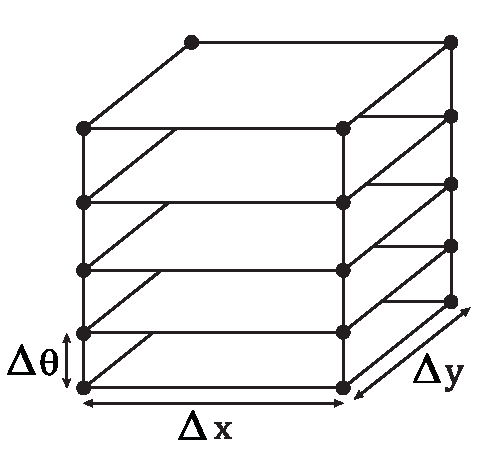
\includegraphics[width=240px]{state_lattice_graphic}
	\caption{A \emph{state lattice} modell egy kis részének diszkretizációja}
	\label{fig:stateLatticeDrawing}
\end{figure}

\begin{explain}
    \Az\told{\ref{fig:stateLatticeDrawing}}+as{} ábrán látható formális paraméterekkel jelölve a diszkretizáció. Ezen paraméterek segítségével egy háromdimenziós térként lehet vizualizálni a \emph{state lattice-t}. Ha a járművet $x$ vagy $y$ irányba mozgatjuk, akkor annak megfelelően az $(x, y)$ síkon mozog. Mivel a járművet a hátsó tengelyének középpontjával tudjuk elhelyezni, a $\theta$ irányú forgatás nem lenne látható. Ezt a problémát oldja meg a harmadik dimenzió, így minden diszkrét $\Delta \theta$ értékhez tartozik egy $(x, y)$ sík. Ezen paraméterek értéke előre meghatározott, például $\Delta x=\Delta y =3cm, \Delta \theta=1$°.
\end{explain}

\subsection{A részekre osztott útvonaltervezés}

Mivel az útvonaltervezőben már adott volt a két pont közti útvonal tervezésének lehetősége, a nagyobb kérdés az maradt, hogy hogyan lehet köztes pontokat meghatározni, amik segítik a jármű haladását és nem teszik sokkal hosszabbá a kapott utat. Ezt a problémát referencia konfigurációk \cite{kug_obp} (később RC) generálásával oldottam meg. Ezek a $[x, y, \theta]^T$ hármasok olyan \emph{state lattice} beli pontok, amelyekhez egy megadott pontból egy egyszerű mozdulat segítségével jutunk. Persze ez a feladat csak akkor "egyszerű" igazán, ha nincsenek akadályok a megadott pont és az RC közt. Ezért az RC-nek nem kell elérhetőnek lennie, és a hozzá vezető útnak sem kell, hogy ütközésmentesen végigjárható legyen. Minden $q_L$ ponthoz (\emph{Landmark}) kettő darab RC generálódik, egy párhuzamos ($q_{RC_P}$) és egy merőleges ($q_{RC_O}$). A két RC a következőképpen írható le:
\begin{align}
    q_{RC_P} &= q_L + 
    \begin{bmatrix}
        \Delta x + \sigma _{xP}\\
        \sigma _{yP}\\
        \sigma _{\theta P}
    \end{bmatrix}\\
    q_{RC_O} &= q_L +
    \begin{bmatrix}
        \Delta x + \sigma _{xO}\\
        \sigma _{yO}\\
        \pm \frac{\pi}{2} + \sigma _{\theta O}
    \end{bmatrix}
\end{align}

Az egyenletben szereplő $\Delta x$ és $\sigma$ paraméterek, amivel a felhasználó személyre szabhatja, hogy hogyan generálódjanak az RC-k. A $\Delta x$ paraméter mondja meg, hogy a járműnek minimum mekkora utat kell megtennie $x$ irányba. A $\sigma$ pedig leírja, hogy a minimális mozgáson felül a három irányba még mennyit haladjon a jármű. Minden $x, y, \theta$ és $P, O$ paraméterhez más $\sigma$ érték tartozik. Például $\sigma _{yP}$ és $\sigma _{yO}$ nagyban eltérnek egymástól, hiszen a merőleges parkoláshoz tartozó nagyobb $\theta$ változást csak nagyobb távon lehet egyszerűen végrehajtani. Ehhez a $\theta$ paraméter és merőleges RC esetén még hozzáadódik $\pm \frac{\pi}{2}$ is attól függően, hogy melyik fordulás van közelebb a cél konfigurációhoz. Az értékek vizualizációja \az\told{\ref{fig:RCDrawing}}+as{} ábrán látható.
\begin{note}
Ideális esetben minden $\sigma$ paraméter egy adott pontosságú intervallum lenne, amiből véletlenszerűen választhatnánk értéket minden RC generálásakor. Ezzel az útvonaltervezőt még jobban tudjuk kényszeríteni, hogy fedezze fel a rendelkezésre álló teret. Mivel beágyazott szoftverben nem előnyös és nehezen megvalósítható (az ipar szabályain belül) a véletlenszámok használata, ezért minden ilyen paraméter egy egyszerű szám, ami járművenként állítható. Az RC-ket a forráskódban ugyanúgy a {\fontfamily{cmtt}\selectfont rbp::pp::common::CPose} osztály valósítja meg, mint a \emph{state lattice} többi pontját.
\end{note}

\begin{figure}[H]
    \centering
	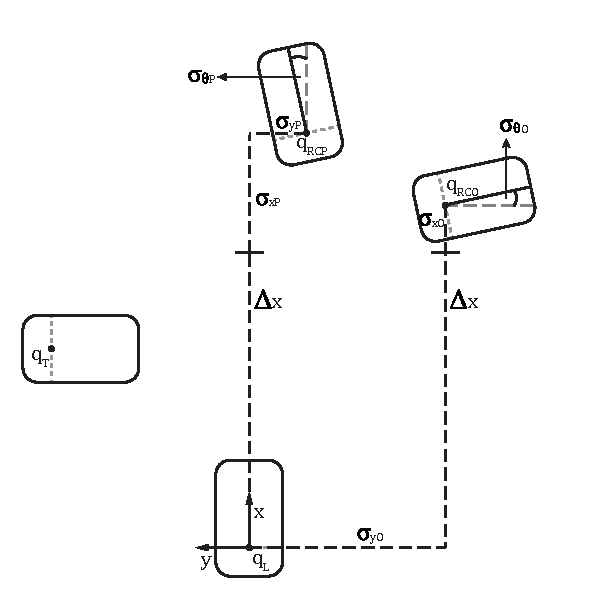
\includegraphics[width=350px]{rc_graphic}
	\caption{$q_L$-hez tartozó $q_{RC_P}$ és $q_{RC_O}$ konfigurációk}
	\label{fig:RCDrawing}
\end{figure}
\clearpage

\section{A projekt limitációi, konvenciók}

Mivel a keretprojekt nagyvállalati környezetben készült, beágyazott rendszerre, ezért sok limitációra, szabványra és kódolási konvencióra figyelemmel kellett lenni a modul elkészítése közben.

\subsection{ISO 16787 és ISO 20900 szabványok}

A szabványok (mint például a címben említett ISO) többek között az aktuális tudásszintet (\emph{State of the Art}) írják le. Ezek a szabványok jogilag nem kötelező érvényűek, azonban, ha a projekt fejlesztése közben nem követünk egy szabványt, akkor egy dokumentált elemzés és indoklás szükséges arra vonatkozóan, hogy a kibocsátott megoldás teljesítménye összehasonlítható a dokumentumban megfogalmazott célokkal. Az ISO 16787 és ISO 20900 szabványok fogalmazzák meg a parkolást segítő- (később APS) és a részben autómata parkolórendszerek (később PAPS) teljesítményének elvárásait és a tesztelésük folyamatát \cite{ISO16787} \cite{ISO20900}. Az APS alapszintű funkcionalitása a következőképpen van megfogalmazva: 
\begin{quote}
    "Az APS felismeri a parkolóhelyet, ahová a járművel parkolni lehet, meghatározza a célparkolási pozíciót, és kiszámítja a parkolás közben bejárandó pályát. Az APS a parkolási manőver során automatikusan vezérli a kormányzást, hogy a járművet a célparkolási pozícióba irányítsa. A vezérlés befejezését követően a jármű helyzetének a célparkolási pozícióhoz viszonyítva meg kell felelnie egy meghatározott pontossági követelménynek."
\end{quote}
 Az útvonaltervező megfelel a megfogalmazott követelmény első felének, hiszen bemeneti adatként megkapja a parkolóhelyet, és benne a célpozíciót is, emellett az ő feladata, hogy kiszámítsa az oda vezető utat. A pontossági követelménynek is eleget tesz a rendszer, hiszen csak akkor tér vissza a teljes útvonallal, ha sikerült a megadott értéken belül lenni a célponttól való eltérésnek.
 \begin{note}
 A kormányzást egy másik \emph{subsystem} végzi azon diszkrét pontok alapján, amelyeket az útvonaltervező kimenetéből származó \emph{Motion Primitive-k} alapján számítottunk ki.
 \end{note}
 Az egyes típusú PAPS egy olyan rendszer, amelyet egy valós személy felügyel a vezető oldali ülésből. Ennek a következő feladatokat kell megvalósítania:
 \begin{itemize}
     \item A rendszert egy hagyományos járművezetőnek kell felügyelnie, aki az autóban ül
     \item A hagyományos járművezetőnek kell kérnie az automatizált parkolási manővert
     \item A rendszer parkolóhelyeket, parkolózónákat és garázsokat keres
     \item A keresés automatikusan vagy a hagyományos járművezető kezdeményezésére is indulhat.  Mindkét esetben a rendszernek tájékoztatnia kell a hagyományos járművezetőt, ha azonosított egy lehetséges parkolóhelyet, parkolózónát vagy garázst
     \item Ha több lehetséges parkolóhelyet, parkolózónát vagy garázst azonosít a rendszer, akkor meg kell jelenítenie a lehetőségeket, és a hagyományos járművezető kiválaszthatja ezek közül a megfelelőt
     \item Ha a hagyományos járművezető nem választ egyet sem a PAPS által azonosított több parkolóhely, parkolózóna vagy garázs közül, a keresés folytatódhat
 \end{itemize}
 Ezen feladatokat is egy másik \emph{subsystem} végzi, ami direkt képes indítani az útvonaltervező modult. A két szabvány definiál még többféle parkolóhelyet is. Az APS esetében ezek az objektumok vagy festett vonalak által határolt parkolóhelyek, és azon belül pedig párhuzamos és merőleges változatok. A PAPS esetében pedig a követelményekben említett parkolóhely, parkolózóna és a parkoló garázs. Az első két típus esetében megfogalmaz külön párhuzamos és merőleges változatokat az APS-hez hasonlóan.

 \subsection{A projektre vonatkozó előírások}

 Ebben a pontban bemutatom a keretprojekt előírásait és a használt technológiákra vonatkozó korlátozásokat. Az első és legfontosabb alapot a statikus kódelemzésre vonatkozó szabályok adják. A szabálykészlet több mint 4000 bejegyzésből áll, melyek változó erősségűek. Ezeket az ISO/IEC 14882:2014(E) szabvány és elődjeik, SEI Cert C++ Coding Standard, és az AUTOSAR Guidelines for C++14 alapján határozták meg a nem definiált és implementációspecifikus működés elkerülésére. Ezzel szemben magára a forráskód nyelvének a frissített ISO/IEC 14882:2017 szabványt kell követni, amely a C++17 megfelelő használatát írja le. A kód felépítésére a következők vonatkoznak:
 \begin{itemize}
     \item Nem használható semmilyen primitív \emph{Assembly} utasítás
     \item Csak \emph{file include} preprocesszor utasítások és \emph{header guard-ok}
     \item Nem használható dinamikus memória
     \item Nem használhatók futási idejű típusinformációk (így nem lehetséges a {\fontfamily{cmtt}\selectfont dynamic\_cast} sem)
 \end{itemize}
 \begin{note}
     Minden \emph{header guard} nevének meg kell egyeznie a \emph{file} nevével, amiben szerepel.
 \end{note}
 
 Mivel nem direkt a standard könyvtárban definiált típusokat használjuk, hanem egy belsős keretrendszer ({\fontfamily{cmtt}\selectfont vfc}, \told{\ref{fig:userInterface}}+as{} táblázat) típusait, ezért a típusozásra is vannak megkötések.
 \begin{itemize}
     \item Minden adattípusnak az alapja a {\fontfamily{cmtt}\selectfont vfc} típusai legyenek (kivétel a {\fontfamily{cmtt}\selectfont void} és {\fontfamily{cmtt}\selectfont bool})
     \item 32 bites \emph{Integer} típus az alapértelmezett minden egész számhoz
     \item Nem használhatóak a C nyelvben használatos tömbök
     \item {\fontfamily{cmtt}\selectfont enum} típusok helyett {\fontfamily{cmtt}\selectfont enum class}
     \item Erős típusozás
     \item Értékek inicializásása a {\fontfamily{cmtt}\selectfont \{\}} operátorral
 \end{itemize}
 Az erős típusozás úgy értendő, hogy az értékek információtartalma a típusban, nem pedig a dokumentációban található. Főleg a valódi mértékegységgel rendelkező értékeknél fontos, hiszen így \emph{type safe} lehet az egész kódbázis.
\begin{table}[h]
    \centering
    \renewcommand{\arraystretch}{1.5} % Adjust row spacing
    \begin{tabular}{ | c | c | }
        \hline
        \textbf{{\fontfamily{cmtt}\selectfont vfc}} & \textbf{Standard C++} \\
        \hline
        \hline
        
        {\fontfamily{cmtt}\selectfont vfc::int32\_t} & {\fontfamily{cmtt}\selectfont int} \\
        \hline
        {\fontfamily{cmtt}\selectfont vfc::int64\_t} & {\fontfamily{cmtt}\selectfont ::std::int64\_t} \\
        \hline
        {\fontfamily{cmtt}\selectfont vfc::uint8\_t} & {\fontfamily{cmtt}\selectfont ::std::uint8\_t} \\
        \hline
        {\fontfamily{cmtt}\selectfont vfc::float32\_t} & {\fontfamily{cmtt}\selectfont float} \\
        \hline
        {\fontfamily{cmtt}\selectfont vfc::size\_t} & {\fontfamily{cmtt}\selectfont ::std::size\_t} \\
        \hline
        {\fontfamily{cmtt}\selectfont vfc::TFixedVector} & {\fontfamily{cmtt}\selectfont ::std::vector} \\
        \hline
    \end{tabular}
    \label{tab:vfcToStd}
    \caption{Néhány standard C++ típus {\fontfamily{cmtt}\selectfont vfc} megfelelője}
\end{table}

 A függvényekre és metódusokra csak annyi a kikötés, hogy rekurzió nem használható.
 \begin{note}
     Kivétel a rekurzió tiltása alól az \emph{overloaded} függvények egymásba ágyazása. Ilyenkor is ugyanazt a függvényt vagy metódust hívjuk önmagán belül, de más paraméterekkel és pontosan ismerjük a \emph{call depth-et}.
 \end{note}
 A külső könyvtárak használata is limitálva van. Csak azok használhatók, amelyek direkt engedélyezve vannak (\emph{whitelist}). A C és C++ standard könyvtárak is külső könyvtárnak minősülnek, ezért a használatuk csak \emph{unit} tesztek 
 és fejlesztői eszközök implementációjában engedélyezett.

 \subsection{Kódolási konvenciók}
 Ebbe az osztályba főleg a névadási és kommentelési szokások egységesítése tartozik. Mind a \emph{file-ok}, változók és osztályok neveire vannak megkötések, ezeket is a projekt és a hozzá tartozó szabványok írják le. A mappa és \emph{file} elnevezésekre a következők vonatkoznak:
 \begin{itemize}
     \item A mappa és \emph{file} nevekben nem szerepelhet nagybetű
     \item A nagybetűk helyett {\fontfamily{cmtt}\selectfont snake\_case} használandó
 \end{itemize}
 Az objektumok elnevezésére a következők vonatkoznak:
 \begin{itemize}
     \item Minden \emph{enum} neve 'E' betűvel jelölendő
     \item Minden osztály \emph{struct} neve 'C' betűvel jelölendő
     \item Minden \emph{template} neve 'T' betűvel jelölendő
     \item Minden \emph{union} neve 'U' betűvel jelölendő
     \item Ha a név több szóból rakódik össze, {\fontfamily{cmtt}\selectfont PascalCase} használandó
 \end{itemize}
 A változókat kódon belül úgy kell elnevezni, hogy egyértelmű legyen a funkciójuk és az értékek, amiket tárolnak. Rövidítések használhatók, például {\fontfamily{cmtt}\selectfont dx, dy} távolságok jelölésére vagy {\fontfamily{cmtt}\selectfont i, it} ciklusváltozóknak. Nem lehet több változónév, amit csak a nagybetűsítés választ el egymástól. Ezen kívül viszont speciális szabályok is vonatkoznak bizonyos változónevekre:
 \begin{itemize}
     \item Osztályon belüli \emph{member-ek} "m\_" előtaggal szerepeljenek
     \item A függvényparaméterek "f\_" előtaggal szerepeljenek
     \item A konstans kifejezések "k\_" előtaggal szerepeljenek
 \end{itemize}
\begin{note}
     A változónevek kiegészíthetőek más elemekkel is, hogy pontosítsuk a jelentést, például {\fontfamily{cmtt}\selectfont m\_heap\_p} egy osztály \emph{heap} adattagjára mutató \emph{pointer}.
\end{note}
A kommentek formájára és tartalmára is vannak konvenciók. Nem használhatók többsoros kommentek, helyette több egysoros kommentre kell tördelni azokat. A {\fontfamily{cmtt}\selectfont //TODO} típusú kommentek használhatók, de csak megfelelő \emph{ticket} számmal ellátva.
\\

\lstset{caption={Példa a megkötéseknek eleget tevő kódra}, label=src:compliantCode}
\begin{lstlisting}[language={C++}]
class CCompliantClass
{
public:
    CCompliantClass() : m_restrictions{}
        {};

    // Adds a restriction to the container
    void addRestriction(const ERestriction f_restriction); 
        //TODO implementation
        //<TICKET-01>

    // Gets all restrictions
    vfc::TFixedVector<ERestriction, k_maxRestrictions> getRestrictions() const;
        //TODO implementation
        //<TICKET-02>

private:
    vfc::TFixedVector<ERestriction, k_maxRestrictions> m_restrictions;
    static constexpr vfc::int32_t k_maxRestrictions{10};
};
\end{lstlisting}
\clearpage

\section{Az útvonaltervező felépítése és működése}

Az első pontban kitértem az összes olyan elméleti részre, ami az útvonaltervező működésének megértéséhez szükséges. Ez a pont egy átvezetés lesz az elmélet és az elkészített C++ implementáció között. Bemutatom az általam elkészített modul tervét és a hozzá tartozó implementációk egy részét, amik szükségesek a teljes felépítés megismeréséhez.

\subsection{A \emph{Waypoint Module} kompozit}

Az általam készített \emph{Waypoint Module} tartalmazza a RC-k generálásához, tárolásához és lekérdezéséhez szükséges logikát. Ezen felül tartalmaz statikus segédfüggvényeket is, amik főleg az RC-k kiszámításánál szükségesek. Minden osztály és (egyéb forráskód is, ahol lehetséges) egy \emph{header} és egy vagy több \emph{source file-ra} van felosztva. Az osztályok és azok metódusai (vagy a statikus függvények definíciói) a megfelelő {\fontfamily{cmtt}\selectfont *.hpp} \emph{file-ban}, míg az implementációk a hozzá tartozó {\fontfamily{cmtt}\selectfont *.cpp} \emph{file-ban}. \emph{Template-et} használó osztályok vagy metódusok esetén az implementáció a {\fontfamily{cmtt}\selectfont *.inl} \emph{file-ban} történik. Erre azért van szükség, mert \emph{template-tel} rendelkező osztályokat vagy metódusokat nem lehet {\fontfamily{cmtt}\selectfont *.cpp} \emph{file-ban} implementálni. Ez azért van, mert a C++ \emph{template-ek} fordítási időben keletkeznek, tehát a \emph{compiler-nek} a teljes definícióra szüksége van, hogy példányosítani tudja őket más fordítási egységekben. Kivétel ez alól a {\fontfamily{cmtt}\selectfont CWaypointModuleParams} osztály, melynek csak \emph{getter} és \emph{setter} függvényei vannak a belső értékekre. Mivel ezek implementációja triviális, ezért a megfelelő {\fontfamily{cmtt}\selectfont .hpp} állományban vannak {\fontfamily{cmtt}\selectfont inline} előtaggal ellátva. Ez azt eredményezi, hogy a fordító minden függvényhívásnál kicseréli a hívást a bennelévő implementációval. Ennek segítségével gyorsabb és hatékonyabb lehet a program, mert a valóságban nincs függvényhívás, tehát nem kell a hozzá tartozó értékeket a \emph{stack-re} tenni és ugrani a függvénytörzshöz és vissza \cite{inline}.

\begin{note}
Lehetséges lenne a {\fontfamily{cmtt}\selectfont *.hpp} \emph{file-okban} már definiálni ezeket a metódusokat, csak olvashatóság miatt vannak különválasztva. Egy másik elfogadott módszer a {\fontfamily{cmtt}\selectfont *.tpp} \emph{file-ok}, de a projekt keretein belül mindenhol az előbb említett módszer van használva.
\end{note}

\begin{figure}[H]
    \centering
	\includegraphics[height=348px]{waypoint_module_folders}
	\caption{A \emph{Waypoint Module} mappaszerkezete}
	\label{fig:waypointModuleFolder}
\end{figure}

A modul összes osztálya és különálló segédmetódusa az {\fontfamily{cmtt}\selectfont rbp::pp::waypoint\_module} \emph{namespace-ben} helyezkedik el, később az osztályok megnevezésénél ezt elhagyom. A legkomplexebb és a számítás nagy részét végző osztály a {\fontfamily{cmtt}\selectfont CReferenceConfigurationCalculator}. Minden másik ebben a kompozitban található osztály az ő működését segíti, vagy teszi lehetővé a benne lévő adatok hatékony tárolását. Az ezen osztályok közötti kapcsolatot a modul osztálydiagramján (\told{\ref{fig:waypointModuleClassDiagram}}+as{} ábra) szemléltetem.

\begin{figure}[H]
    \centering
	\includegraphics[width=1\textwidth]{waypoint_module_class}
	\caption{A \emph{Waypoint Module} osztálydiagramja}
	\label{fig:waypointModuleClassDiagram}
\end{figure}

Az RC-k kiszámítása során ezek az osztályok statikus segédfüggvényeket is használnak. Ezek nincsenek osztályokba szervezve, hiszen semmi olyan adattal nem dolgoznak, amihez enkapszuláció szükséges. Főleg geometriai transzformációkat valósítanak meg. Mivel ezek a metódusok nem tartoznak osztályokba, a tesztelhetőségük is könnyebb. A koordináta-rendszer transzformációkra is azért van szükség, mert az útvonaltervező koordináta-rendszerének a központja nem a jármű hátsó tengelyének középpontjában van, de az RC-knél a számítást megnehezítené, ha ugyanazt a központot használnánk.
\clearpage

\lstset{caption={A \emph{Waypoint Module} segédfüggvényei}, label=src:waypointHelpers}
\begin{lstlisting}[language={C++}]
#include "rbp/pp/common/common_math_utils.hpp"
#include "rbp/pp/common/common_posture.hpp"
#include "vfc/core/vfc_math.hpp"

namespace common = rbp::pp::common;

namespace rbp::pp::waypoint_module
{
/// @brief Transforms a global pose to the vehicle's local coordinate system. (0, 0, 0) is the rear axle point of the vehicle and the x axis is is in the direction the vehicle is facing.
common::CPose transformToLocalPose(const common::CPose& f_pose, const common::CPose& f_requestOrigin);

/// @brief Transforms pose in the vehicle's local coordinate system to a global pose.
common::CPose transformToGlobalPose(const common::CPose& f_pose, const common::CPose& f_localOrigin);

} // namespace rbp::pp::waypoint_module
\end{lstlisting}

\begin{note}
A fejlesztési szakasz elején, az RC-k generálásához készültek vizualizációs Python \emph{script-ek}. Ebben a szakaszban derült ki, hogy a koordináta-rendszerek közti váltás könnyebben implementálható, és átláthatóbb, mint a folyamatos globális rendszerben történő számítás. A másik lehetőség az volt, hogy a jármű állása alapján $x$ és $y$ irányú komponensekre bontjuk a $\Delta x$ minimális elmozdulás paramétert, és kvadránsokbeli állások szerint előjelezzük a $x, y, \sigma$ paramétereket. Ezek nagy hibafaktort és sok helyen nem várt működést eredményeztek, és nem sokkal voltak algoritmikusan hatékonyabbak, mint a végső implementáció.
\end{note}
\clearpage

\subsection{A \emph{heap} adatszerkezet szerepe}

A {\fontfamily{cmtt}\selectfont CReferenceConfigurationCalculator} osztály szerepe nem csak az RC-k generálása, hanem ezek tárolása és megfelelő kezelése is. Mikor a felhasználó hozzáad egy új \emph{landmark-ot}, a célpont segítségével kiszámolható egy becslés, ami leírja, hogy mennyire nehéz eljutni a felajánlott ponttól a célig. Minnél nagyobb az érték, annál költségesebb a járműnek megtenni az utat. Ezt az értéket a {\fontfamily{cmtt}\selectfont CReferenceConfigurationCalculator::calcCost} függvény számolja a következő módon \cite{kug_obp}:
\begin{align}
    c_L &= d_L^T \times R \times d_L + r_LP_l + r_{DC} N_{DC_L}
\end{align}
Az egyenletben $d_L \in \mathbb{R}^{1 \times 3}$ jelöli a megadott \emph{landmark} és a célpont közti eltérést, $R \in \mathbb{R}^{3 \times 3}$ egy diagonális súlymátrix, ami segít, hogy az $x, y$ és $\sigma$-beli eltérések a jármű fizikai határait figyelembe véve számítsanak a költségbe. Továbbá $P_L$ jelöli az útvonal hosszát, és $r_L$ a hozzá tartozó súlyparaméter. Ugyanígy $N_{DC}$ a \emph{landmark} eléréséhez szükséges irányváltások száma és $r_{DC}$ a hozzá tartozó súlyparaméter. Ezen paraméterek alapértelmezetten a következők:
\begin{table}[htb]
	\centering
	\begin{tabular}{ | c | c | c | }
		\hline
		\multirow{2}{*}{\textbf{Paraméter jelölése}} & \multicolumn{2}{ c | }{\textbf{Paraméter értéke}} \\
		\cline{2-3}
		& Érték & Mértékegység\\
		\hline \hline		
		$r_L$ & 10 & $m^{-1}$ \\
		\hline
		$r_{DC}$ & 50 & -  \\
		\hline
		$R_{1,1}$ & 0,1 & $m^{-2}$ \\
		\hline 
		$R_{2,2}$ & 1 & $m^{-2}$ \\
		\hline 
		$R_{3,3}$ & 3,5 & $rad^{-2}$ \\
		\hline 
	\end{tabular}
	\caption{Alapértelmezett súlyértékek költségszámításhoz}
	\label{tab:defaultCostParams}
\end{table}

A tárolt \emph{landmark-ok} tehát a számított költség szerint sorbarendezve kell, hogy legyenek. Ennek a problémának a megoldását a \emph{heap} adatszerkezet adja. Az implementációban a \emph{min binary heap} \cite{min_heap} változatát valósítottam meg, melynek lényege, hogy a legkisebb tárolt érték a \emph{heap} tetején helyezkedik el. A legfontosabb műveletek (\emph{insert, pop/peek, push}) mind a legrosszabb esetben is $O(\log n)$ műveletigényűek, így az adatszerkezet megfelelően hatékony a \emph{landmark-ok} tárolására és lekérdezésére. A C++ implementáció a \ref{fig:waypointModuleClassDiagram} osztálydiagram alapján egy tömbbel van ábrázolva, melyben a szülők és a bal, illetve jobb gyerekeik kötött helyen szerepelnek. 
\clearpage

\lstset{caption={Index számítás egy tömb alapú \emph{heap-ben}}, label=src:heapIndexes}
\begin{lstlisting}[language={C++}]
static vfc::int32_t parentIndex(vfc::int32_t f_index)
{
    return (f_index - 1) / 2;
};

static vfc::int32_t rightChildIndex(vfc::int32_t f_index)
{
    return (2 * f_index + 1);
};

static vfc::int32_t leftChildIndex(vfc::int32_t f_index)
{
    return (2 * f_index + 2);
};
\end{lstlisting}

A \emph{heap-et} ábrázoló tömbben tartjuk az osztályban jelölt \emph{template} szerint a {\fontfamily{cmtt}\selectfont HeapElementType} típusú objektumokat, amik a modulon belül {\fontfamily{cmtt}\selectfont THeapElement<common::CPose>} objektumok. A {\fontfamily{cmtt}\selectfont THeapElement} osztály a neki megadott \emph{template} argumentumot egészíti ki egy költségértékkel, ami szerint sorbarendezhetők az adott példányok.

\subsection{Együttműködés az útvonaltervezővel}

Az útvonaltervezést a C++ implementációban a {\fontfamily{cmtt}\selectfont CStateLatticePlanner} osztály végzi. Ennek az objektumnak az adattagjai között szerepel az előző alpontban tárgyalt \emph{Waypoint Module} {\fontfamily{cmtt}\selectfont CReferenceConfigurationCalculator} osztályának egy példánya is. Miután a felhasználó beállította a megfelelő bemeneti adatokat, a {\fontfamily{cmtt}\selectfont CStateLatticePlanner::planPath} (\told{\ref{fig:userInterface}}+as{} kódrészlet) API metódus meghívásával indítható el a tervezés. Az eredményt \emph{Motion Primitive-ek} formájában kapjuk meg, amit bemeneti paraméterként adunk át a függvénynek. Itt csak akkor használja a rendszer a részekre osztott parkolás módszerét, ha ez engedélyezve van a tervező paramétereiben. \clearpage

\lstset{caption={A {\fontfamily{cmtt}\selectfont CStateLatticePlanner::planPath} függvény}, label=src:planPath}
\begin{lstlisting}[language={C++}]
template <class TConfig>
bool CStateLatticePlanner<TConfig>::planPath(MotionPrimitiveResultVector& f_primitivesFromEndToStart) {
    m_pathDatabase.clear();
    this->m_input.setStartAndTargetCollisionRelevancy(true);
    auto planningSuccessful = planFromAToB(f_primitivesFromEndToStart);
    
    if (!planningSuccessful && this->m_ppParams.get<config::CEnableWaypointModuleParams>()) {
        this->m_input.setIterationLimit(1250);
        const auto isFlippedPlanning = CPathPlanner<TConfig>::m_input.isPlanningDirectionFlipped();
        
        if (isFlippedPlanning) {
            m_configurationCalculator.reInit(
                this->m_input.getTargetArea().getTargetPosture().pose(), this->m_input.getStartPosture().pose());
        }
        else {
            m_configurationCalculator.reInit(
                this->m_input.getStartPosture().pose(), this->m_input.getTargetArea().getTargetPosture().pose());
        }
        planningSuccessful = handlePlaningWithWaypoints(f_primitivesFromEndToStart);
    }
    this->m_input.setIterationLimit(CStateLatticePlannerConstants::k_nodeExpansionIterationLimit);
    
    return planningSuccessful;
}
\end{lstlisting}
\clearpage

A két pont közötti útkeresést a  {\fontfamily{cmtt}\selectfont CStateLatticePlanner::planFromAToB} függvény végzi, aminek a ugyanúgy bemeneti paraméterként adjuk át az útvonalat tartalmazó vektort. Ezen kívül visszatér egy logikai értékkel is, hogy sikeres volt-e a tervezés. Ha a felhasználó igénybe szeretné venni a \emph{Waypoint Module} funkcionalitását is, akkor a többrészes tervezést a {\fontfamily{cmtt}\selectfont CStateLatticePlanner::handlePlaningWithWaypoints} függvény végzi, ami ugyanúgy paraméterezett és ugyanolyan visszatéréssel rendelkezik, mint az előbb említett metódus. Ilyenkor az útvonalkeresés algoritmusa a következő:

\begin{algorithm}[H]
\caption{Az útvonalkeresés algoritmusa}
\label{alg:planPath}
\textbf{\underline{Funct}} planPath
\begin{algorithmic}[1] % sorszámok megjelenítése minden n. sor előtt, most n = 1
\State Plan from $q_S$ to $q_T$
\If{planning failed}
    \For{$i=1..N_w$}
    	\State Calculate $q_L, q_{RCP}, q_{RCP}$ 
    	\State Plan from $q_L$ to $q_{RCP}$ and $q_{RCO}$
    	\State Calculate $q_{closest}$ and $N_{DC}$ for both configurations
    	\State Save path from $q_L$ to $q_{closest}$ for both configurations
    	\State Plan from both $q_{closest}$ points to $q_T$
    	\If{planning successful from any $q_{closest}$ to $q_T$}
    	  \State Save path from $q_{closest}$ to $q_T$
            \State Request full path from database
            \State \textbf{break}
        \Else
    	  \State Add $q_{RCP}, q_{RCO}$ and all direction change points as landmarks
    	\EndIf
    \EndFor
\EndIf
\State \textbf{return} $\top$ if planning successful, else $\bot$
\end{algorithmic}
\end{algorithm}

Az algoritmusban a $N_w$ paraméter a maximálisan generálható \emph{waypoint-ok} számát írja le. Ennek az értéknek a megválasztása fontos, hiszen ha túl alacsonynak választjuk, akkor nem hagyjuk, hogy az útvonaltervező eléggé felfedezze a rendelkezésre álló teret. Ha viszont túl magas értéknek választjuk, akkor a futási időt erősen megnöveli.

\begin{note}
Az implementációban ez az érték $N_w = 10$-nek van választva. Fontos volt még, hogy ahogy növeljük a maximálisan generálható \emph{waypoint-ok} számát, hasonlóan csökkentsük a belső A* algoritmus maximális iterációszámát, hiszen legrosszabb esetben $2N_w+1$ tervezés történhet az algoritmus során.
\end{note}

A másik fontos érték az algoritmusban a $q_{closest}$ pont. Mivel a generált RC-knek nem kell elérhetőnek lenniük, számon kell tartsuk a célhoz legközelebbi pontot, amit elért az algoritmus. Emellett még kezelnünk kell, hogy akkor is engedjük a tervezést, ha a \emph{waypoint} direkt ütközésben van egy objektummal. Erre azért van szükség, mert az útvonaltervező végez egy ellenőrzést minden tervezés előtt, hogy a start és célpozíció nincsenek-e ütközésben. Ezt minden RC-hez való tervezés előtt ki kell kapcsolni, hogy megfelelő utat kapjunk. Ezt a kapcsolót is az \emph{input-ban} tudjuk állítani a {\fontfamily{cmtt}\selectfont setStartAndTargetCollisionRelevancy} függvény segítségével.

\begin{figure}[H]
	\includegraphics[width=1\textwidth]{waypoint_module_component}
	\caption{Az útvonaltervező komponensdiagramjának egy része}
	\label{fig:plannerComponentDiagram}
\end{figure}

\begin{explain}
    Az előző ábrán az útvonaltervező a dolgozat szempontjából releváns részeit tartalmazza, a hozzájuk tartozó kapcsolatokkal és \emph{input/output-okkkal}. Ezen kívül sok másik belső komponens építi fel, de ezeket helymegtakarítás és titoktartás szempontjából nem ábrázoltam.
\end{explain}

\subsection{Az útvonalrészletek tárolása}

A $q_L$ és $q_{RC}$ pontok közötti szakaszokat el kell menteni, hogy a tervezés végén rekonstruálni lehessen a teljes útvonalat. Ezt a feladatot a {\fontfamily{cmtt}\selectfont CPathDatabase} osztály látja el. Az osztály egy fában tárolja a megadott \emph{landmark-okat} és az őket összekötő útszakaszokat. A gráf egy \emph{map} típusú tárolóval van megvalósítva, melynek kulcsa az út végpontja ($q_{closest}$ vagy egy esetben $q_T$), és a hozzá tartozó érték egy $[q_L, P_{L \implies closest}]^T$ páros, ahol $P_{L \implies closest}$ jelöli a \emph{landmark} és a hozzá tartozó $q_{closest}$ pont közötti utat ábrázoló \emph{Motion Primitive} vektort.

\begin{figure}[H]
    \centering
	\includegraphics[width=220px]{images/path_database.jpg}
	\caption{{\fontfamily{cmtt}\selectfont CPathDatabase} egy lehetséges belső szerkezete}
	\label{fig:pathDatabase}
\end{figure}

A fában a csúcsok jelölik a \emph{landmark-okat}, és az őket összekötő élek pedig a köztük lévő utat. Minden csúcsnak maximum 4 gyereke lehet. Ebből 2 akkor jön létre, amikor az adott $q_i$ pontot választjuk a következő \emph{landmark-nak}. Ha a kiszámított RC-hez több mozdulatból jutunk el, akkor az egyik gyerek nem közvetlenül a generált RC, hanem a hozzá vezető első mozdulat vége. Ha egy ilyen köztes pontot választunk kiterjesztésre, akkor $q_i$-nek a művelet után már három gyereke van. Ha ebből a pontból elérhető a célpont is, akkor 4 gyereke lesz $q_i$-nek. Egy fa építésére példát a \ref{fig:treeBuilding} ábrán mutatok be. 

\begin{note}
A 4 gyerekes csúcs csak elméletben lehetséges, hiszen nem terjesztünk ki azután csúcsot, hogy megtaláltuk a $q_T$-be vezető utat. Gyakorlatban $q_T$ mindig a legalsó szinten szerepel, és nincs testvére.
\end{note}

\begin{figure}[H]
    \centering
	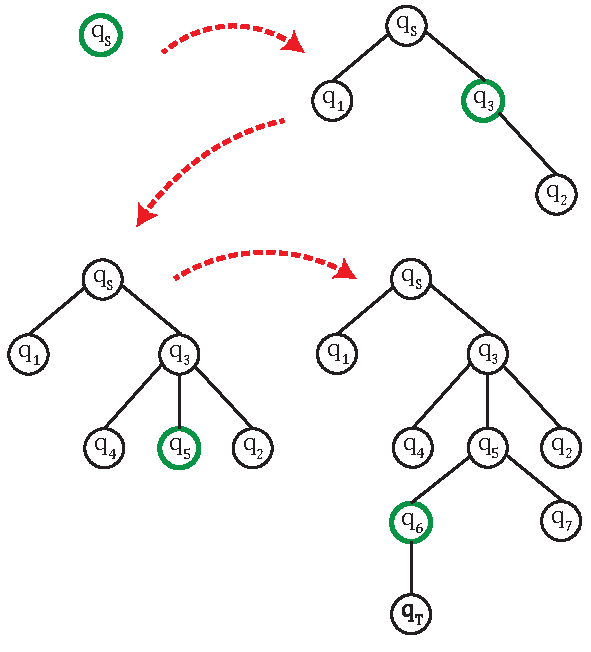
\includegraphics[width=300px]{images/path_database_build_process.pdf}
	\caption{A fa építésének folyamata}
	\label{fig:treeBuilding}
\end{figure}

\begin{explain}
A példában a $q_S$ pontot helyezzük először az adatbázisba, így az lesz a fa gyökere. Mivel ez az egyetlen pont, amit ki tudunk terjeszteni, ezt használjuk \emph{landmark-nak}. Ennél a kiterjesztésnél kerülnek a fába a $q_1, q_2, q_3$ pontok. Ezek közül $q_1$ és $q_2$ a két generált RC, és $q_3$ az egyikhez vezető úton egy irányváltási pont. A költségszámítás alapján a következő legkedvezőbb pont $q_3$, tehát kiterjesztjük, így megkapjuk a két RC-t: $q_4$-et és $q_5$-öt. Ez alkalommal nem kellett irányt váltani a \emph{waypoint-hoz} vezető úton, így nem keletkezik köztes pont. A következő lépésben a $q_5$ RC-t használjuk, hogy újabb \emph{waypoint-okat} generáljunk, ezek lesznek $q_6$ és $q_7$. Ebben a lépésben találjuk meg a $q_T$ célpontot is a $q_6$ RC-ből kiindulva, ezért $q_6$ egyetlen gyereke $q_T$ lesz.
\end{explain}

Ezen kívül a {\fontfamily{cmtt}\selectfont CPathDatabase} osztály feladata még az uniform méretű \emph{Motion Primitive-ek-en} kívüli dinamikus hosszúságú mozdulatok hosszú távú tárolása is. Erre azért van szükség, mert az útvonaltervező eredeti implementációjában ezek minden tervezés után törlődtek. Mivel a \emph{Waypoint Modul} használatával legjobb esetben is 2 tervezés történik, szükség van ezek mentésére.
\clearpage

A tárolást megvalósító C++ implementáció a {\fontfamily{cmtt}\selectfont CConnectingPrimitiveContainer} osztály. Ilyen típusú objektumokat tárol a {\fontfamily{cmtt}\selectfont CPathDatabase} osztály egy, az előzőnél egyszerűbb \emph{map}-ban. \\

\lstset{caption={A {\fontfamily{cmtt}\selectfont CConnectingPrimitiveContainer} osztály}, label=src:connPrimiContainer}
\begin{lstlisting}[language={C++}]
class CConnectingPrimitiveContainer
{
public:
    CConnectingPrimitiveContainer() = default;

    CConnectingPrimitiveContainer(const CConnectingPrimitiveContainer& f_other);

    void addPrimitive(const CMotionPrimitiveBase* f_primitive);

    vfc::TFixedVector<const CMotionPrimitiveBase*, 5> getPrimitivePointers() const;

private:
    vfc::TFixedVector<CCircleMotionPrimitive, 4>      m_circlePrimitives;
    vfc::TFixedVector<CLineMotionPrimitive, 1>        m_linePrimitives;
    vfc::TFixedVector<const CMotionPrimitiveBase*, 5> m_primitivePointers;
};
\end{lstlisting}

Mivel a \emph{Motion Primitive-ek} absztrakt ősosztály segítségével vannak implementálva, ezért nem lehet őket direkt példányosítani. A belőlük leszármazó {\fontfamily{cmtt}\selectfont CLineMotionPrimitive} és {\fontfamily{cmtt}\selectfont CCircleMotionPrimitive} objektumokat példányosítjuk, és a rájuk mutató \emph{pointer-eket} adjuk vissza lekérdezés esetén. Azt, hogy egy \emph{Motion Primitive} melyik kategóriába esik, a primitív $\delta$ paramétere alapján tudjuk eldönteni, hiszen az egyenes irányú mozgáshoz nem szükséges kormányszöget változtatni. Ezen felül szükséges még felülírni az osztályhoz tartozó \emph{copy constructor-t}, mert másolás esetén a régi objektum \emph{pointer-eit} fogja tárolni az eredmény, ami érvénytelen hivatkozásokat eredményez.
\clearpage

\begin{note}
Mind a dinamikus hosszúságú primitívek tárolása, és a leszármazott osztályok példányosítása is azért szükséges, mert a projekt keretein belül nem használható dinamikus memória. Ellenkező esetben a {\fontfamily{cmtt}\selectfont new} kulcsszó segítségével könnyebben kezelhető lenne a \emph{Motion Primitive-ek} tárolása. Ilyenkor viszont figyelni kell, hogy a {\fontfamily{cmtt}\selectfont delete}-t használjuk a foglalt memóriának a felszabadítására. A C++ nyelvben több lehetőség is lenne ennek automatizálására, az itt megfelelő módszer az {\fontfamily{cmtt}\selectfont std::shared\_ptr} lenne, amely automatikusan törlődik, ha az összes őt birtokló objektum is törlődik. \cite{shared_ptr}
\end{note}

\section{Tesztelés}

Ebben a pontban bemutatom az általam készített programkönyvtár tesztelésének lépéseit. A \emph{unit test-ek} készítéséhez a \emph{Google Test} tesztkeretrendszert használtam, a bonyolultabb integrációs teszteket pedig a projekt saját vizualizációs szoftverében végeztem.

\subsection{Tesztelési terv}

Ahhoz, hogy a magasabb absztrakciós szinten lévő osztályok megfelelően működjenek, a legfontosabb tesztelni az őket segítő metódusokat. Ezt valósítja meg a {\fontfamily{cmtt}\selectfont waypoint\_module\_helpers\_test.cpp} \emph{file}. Minden segédfüggvényhez definiáltam ekvivalenciaosztályokat, melyekben az elvárt működés ugyanaz. Ezek a forgatásokban jelennek meg: $[0, 2\pi]$, $(2\pi, +\infty)$, $(-\infty, 0)$. Ezekből elég csak osztályonként egy tesztesetet vizsgálni, mert a viselkedésük megegyezik. A koordináta-transzformációs függvényekhez a tesztesetek a következők:
\begin{itemize}
	\item Ha a kért középpont és a valós középpont megegyezik, akkor az eredeti pontot adjuk vissza eredményként
    \item Ha a kért középpont és a valós középpont közt csak eltolás van, akkor az eredmény is helyesen van eltolva
    \item Ha a kért középpont és a valós középpont közt eltolás és forgatás is van, akkor az eredmény is helyesen van transzformálva - forgatás $[0, 2\pi]$
    \item Ha a kért középpont és a valós középpont közt eltolás és forgatás is van, akkor az eredmény is helyesen van transzformálva - forgatás $(2\pi, +\infty)$
    \item Ha a kért középpont és a valós középpont közt eltolás és forgatás is van, akkor az eredmény is helyesen van transzformálva - forgatás $(-\infty, 0)$
\end{itemize}
Ezeken kívül a \emph{heap} adatszerkezet \emph{unit} tesztelése volt még fontos, hiszen a legjelentősebb tároló, ami nem egyértelműen működik (vagy adott a működése, mint például a {\fontfamily{cmtt}\selectfont vfc::TFixedMap} típus). A \emph{heap} metódusainak tesztesetei a következők:
\begin{itemize}
	\item Létrehozáskor üres
	\item Ha adatot adunk hozzá, az adat a tömbben van
	\item Ha kiürítjük a tárolót, akkor újra üres
	\item Ha van elem a \emph{heap-en}, \emph{pop} művelet után az elemek száma csökken
	\item Ha több elemet adunk hozzá, az elemek növekvő sorrendben vannak
	\item Ha ugyanazt az elemet többször adjuk hozzá, a másolat is jelen van
\end{itemize}
A következő osztály, amelynek a működését vizsgálni kell, a {\fontfamily{cmtt}\selectfont CPathDatabase}. A tesztesetek a következők:
\begin{itemize}
	\item Ha egy útvonalat eltárolunk, helyesen kapjuk vissza
    \item Ha tele van az adatbázis, nem tárol el több adatot, de nem ad hibát
    \item Ha kiürítjük az adatbázist, a mérete 0
    \item Ha a teljes útvonalat kérjük, helyesen illeszti a részleteket egymás után
    \item Ha használ a \emph{planner} többrészes tervezést, a valóban használt \emph{waypoint-okat} adja vissza
\end{itemize}
\begin{explain}
    A második teszteset azért szükséges, mert fix méretű \emph{map-pal} dolgozik az osztály. Ennek a mérete úgy van megválasztva, hogy megfelelő használat mellett nem kerülhet bele több elem, mint a maximális méret.
\end{explain}
A {\fontfamily{cmtt}\selectfont CReferenceConfigurationCalculator} működését \emph{unit} tesztelni nehéz, ezért ezt integrációs teszt formájában tesztelem vizualizációs szoftverben. Így könnyebben látható, hogy tényleg jól generálódnak az RC-k, és valóban azok között tervez a rendszer. Egy másik megközelítés a teljes osztály \emph{mock-olása} lenne, hogy minden alkalommal egyszerűen vizsgálható eredményt adjon vissza.

\subsection{Integrációs tesztek, vizualizálás}

Ebben az alfejezetben mutatom be a \emph{Waypoint Module} integrálásának a folyamatát a vizualizációs szoftverbe. Nem szükséges hozzáadni a modult a vizualizációs program \emph{CMake file-jához}, mert az útvonaltervezőn keresztül el lehet érni a szükséges adatokat.

Hogy aktiválni lehessen a többrészes útvonaltervezést, a felhasználói felületen hozzáadtam egy \emph{checkbox-ot} a \emph{"Planner"} beállítási oldalra. Ez a háttérkódban a {\fontfamily{cmtt}\selectfont visualization\_options.hpp} \emph{file-ban} bevezettem egy értéket, ami nyilvántartja, hogy mi a kapcsoló állása. Egy megfelelő getter függvény is tartozik hozzá, ennek segítségével lehet lekérdezni a változó értékét. Ezután ugyanilyen módon hozzáadtam a felhasznált \emph{waypoint-ok} kirajzolásának lehetőségét is. A két paramétert feliratkoztattam a két \emph{checkbox clicked} eseményére.
\\

\lstset{caption={Paraméterek feliratkoztatása az eseményekre 1.}, label=src:connectParams1}
\begin{lstlisting}[language={C++}]
connect(
    f_ui->checkBox_waypoints,
    &QCheckBox::clicked,
    this,
    [=, &f_sceneFrame]
    {
        onVisualisationOptionClicked(f_ui->checkBox_waypoints, &m_showWaypoints);
        f_sceneFrame.redrawWaypoints();
    }
);
connect(
    f_ui->checkBox_waypointModule,
    &QCheckBox::clicked,
    this,
    [=] 
    { 
        onVisualisationOptionClicked(f_ui->checkBox_waypointModule, &m_enableWaypointModule);
    }
);
\end{lstlisting}

A következő feladat az útvonaltervező modul paramétereinek megfelelő beállítása volt a vizualizációs opciók alapján. Ezt is a megfelelő \emph{checkbox clicked} eseményére való feliratkozással értem el. A program futása közben lehetőség van kiírni üzeneteket a konzol ablakba, hogy nyomon lehessen követni, milyen események történnek működés közben. Ezt a {\fontfamily{cmtt}\selectfont qInfo} függvénnyel lehet megtenni.
\\

\lstset{caption={Paraméterek feliratkoztatása az eseményekre 2.}, label=src:connectParams2}
\begin{lstlisting}[language={C++}]
connect(
    ui->checkBox_waypointModule,
    &QCheckBox::clicked,
    this,
    [=]
    {
        m_inputHandler.setEnableWaypointModuleParam(m_visualisationOptions.isWaypointModuleEnabled());
        qInfo(
            m_visualisationOptions.isWaypointModuleEnabled()
            ? "Waypoint Module enabled"
            : "Waypoint Module disabled"
        );
    }
);
\end{lstlisting}

Szükséges volt még a mozgást leíró paraméterek beállítására is lehetőséget biztosítani. Ezt értékenként egy \emph{input} mezővel valósítottam meg a felhasználói felületen, míg a háttérkódban létrehoztam egy {\fontfamily{cmtt}\selectfont WaypointModuleParams struct}-ot. Ezeket az értékeket feliratkoztattam az \emph{input} mezők \emph{textChanged} eseményére, így mindig változnak, ha a felhasználói felületen is változtatnak rajta. Ezeket az értékeket konvertálom tervezés előtt egy, a \emph{Waypoint Module-ban} is használt {\fontfamily{cmtt}\selectfont CWaypointModuleParams} objektumra.

Az útvonaltervező futása után a program lekérdezi a használt \emph{waypoint-okat} és elmenti azokat, hogy kérésre ki lehessen rajzolni a \emph{canvas-ra}. A program alapértelmezetten kikapcsolva tartja a \emph{Waypoint Module-t}.
\clearpage

A {\fontfamily{cmtt}\selectfont CReferenceConfigurationCalculator} osztály tesztelését is a vizualizációs szoftverben végeztem, mert itt jobban látható az RC-k megfelelő generálása. A funkcionalitás vizsgálatához létrehoztam egy {\fontfamily{cmtt}\selectfont test.json} állományt, melyben egy egyszerű \emph{scene-t} definiáltam. Ebben kikényszerítem az útvonaltervezőnél, hogy használjon többrészes tervezést azzal, hogy a jármű elé teszek egy magas objektumot. Mivel az A* algoritmus a megadott iterációszámmal nem tudja kikerülni, ezért életbe lép a \emph{Waypoint Module}. A különböző orientációkat a mozgást leíró paraméterek változtatásával, míg az irányokat az objektum- és a start/cél pozíció mozgatásával tudtam tesztelni. A következő két ábrán a párhuzamos RC-k generálásának a tesztesetei láthatók a startpozíció előtti, illetve mögötti céllal.

\begin{figure}[H]
	\includegraphics[width=1\textwidth]{test_forward}
	\caption{Az első teszteset (előremenet)}
	\label{fig:intTestFor}
\end{figure}

\begin{figure}[H]
	\includegraphics[width=1\textwidth]{test_back}
	\caption{A második teszteset (hátramenet)}
	\label{fig:intTestBack}
\end{figure}

\section{Egyéb felhasznált technológiák}

Ebben a részben a modul elkészítéséhez és működéséhez szükséges egyéb technológiákat is ismertetem. Mivel az alapot képző projekt nagyvállalati környezetben készült, sok keretrendszer és megoldás adott volt, és a megfogalmazott irányelveket követni kellett.

\subsection{\emph{Python} prototípus}

Egy előző megjegyzésben már szerepelt, hogy a valódi implementáció előtt Python prototípus készült az RC-k generálásához és vizualizálásához. Ebben könnyebb volt tesztelni és gyors javításokat végezni, mert nem kellett követni benne a szoros kódolási konvenciókat. E mellett segítette még a prototipizálást, hogy a Python nyelvhez rengeteg bárki számára elérhető könyvtár van szinte bármilyen feladat megoldására. Ezek közül a legfontosabbak számomra a {\fontfamily{cmtt}\selectfont NumPy} és a {\fontfamily{cmtt}\selectfont PyPlot} könyvtárak voltak. Az előbbi a matematikai számítások (például költségszámításnál mátrixszorzás) egyszerűsítésére volt hasznos, míg az utóbbi a vizualizálást segítette. \\

\lstset{caption={A költségszámítás prototípusa Python-ban}, label=src:calcCostPy}
\begin{lstlisting}[language={Python}]
def calc_cost(landmark, start_pose, path_length, direction_changes):
    r_l = 10.
    r_SP = 50.
    r_u = 0.1
    r_v = 1.
    r_theta = 3.5
    R_L = np.diag([r_u, r_v, r_theta])
    e_qL = np.array([0., 0., 0.])
    
    local_x, local_y = common.translate_to_local(start_pose[0], start_pose[1], landmark[0], landmark[1], landmark[2])
    e_qL[0] = abs(local_x)
    e_qL[1] = abs(local_y)
    e_qL[2] = min(abs(start_pose[2] - landmark[2]), common.constrain_angle_to_2pi(start_pose[2] - landmark[2]))

    return np.matmul(np.matmul(e_qL, R_L), e_qL) + r_l * path_length + r_SP * direction_changes
\end{lstlisting}

A forráskódban látszik, hogy a {\fontfamily{cmtt}\selectfont NumPy} csomagban adott a mátrixszorzás, diagonális mátrix képzés és a vektorok összeadása is, így ezek implementálásával nem kellett időt tölteni. A másik feladat az RC-k vizualizálása volt, amihez pedig szükség volt a jármű ábrázolására, forgatására és eltolására. A járművet pontok vektoraként ábrázoltam, így a {\fontfamily{cmtt}\selectfont PyPlot} ki tudja rajzolni azt, és a transzformációk is könnyen elvégezhetők. Ezek a metódusok a {\fontfamily{cmtt}\selectfont plot.py} \emph{file-ban} vannak definiálva.

\begin{figure}[H]
    \centering
	\includegraphics[width=300px, height=290px]{images/rc_30.png}
	\caption{{\fontfamily{cmtt}\selectfont plot.py} kimenete egy adott $\theta$ szöghöz}
	\label{fig:plotPyOutPut}
\end{figure}

\subsection{\emph{CMake build} rendszer}

Mivel a keretprojekt beágyazott rendszerre készül, és \emph{Linux} rendszeren van tesztelve, szükség van egy \emph{cross-platform build} rendszerre. Ezt a feladatot a \emph{CMake} végzi. Minden kompozitnak külön {\fontfamily{cmtt}\selectfont CMakeLists.txt} \emph{file-ja} van, amiben az adott modul függőségeit és felhasznált forráskódjait írjuk le. Így \emph{rebuild} esetén elég csak azt a kompozitot, és annak is csak azon részét újrafordítani, amiben a módosítást végeztük. E mellett képes a rendszer külön \emph{Debug} és \emph{Release build-eket} készíteni, amik fontosak a tesztelésnél. Minden \emph{unit} tesztcsomaghoz is külön {\fontfamily{cmtt}\selectfont CMakeLists.txt} tartozik, hogy mindegyikhez külön futtatható állományt tudjunk készíteni.
\clearpage

\lstset{caption={A \emph{Waypoint Module} CMakeLists.txt \emph{file-jának} felépítése}, label=src:cmakeLists}
\begin{lstlisting}[language={make}]
set(LIB_NAME waypoint_module)

set(TARGET_NAME ${LIB_NAME})
add_library(${TARGET_NAME})

add_library(${PROJECT_NAME}::${LIB_NAME} ALIAS ${TARGET_NAME})

target_link_libraries(${TARGET_NAME}
    PRIVATE
    PUBLIC vfc::vfc rbp_pp::common
)

target_sources(${TARGET_NAME} PRIVATE "src/reference_configuration_calculator.cpp" "src/waypoint_module_helpers.cpp")

target_include_directories(${TARGET_NAME} PUBLIC "inc")

install(TARGETS ${TARGET_NAME} LIBRARY DESTINATION lib)
install(DIRECTORY "inc/" DESTINATION "include/${TARGET_NAME}")

if(NOT DEFINED DISABLE_UTF)
    add_subdirectory(test/unit_test)
endif()

set_target_properties(${TARGET_NAME} PROPERTIES rb_export_as_package_component ${PROJECT_NAME}::${TARGET_NAME})
\end{lstlisting}
\clearpage

\subsection{Verziókezelés}
Mind a C++ implementáció, mind a \emph{Python} prototípus elkészítésének segítésére a {\fontfamily{cmtt}\selectfont Git} verziókezelő rendszert használtam. Az előbbi tárolását a Robert Bosch Kft. által biztosított és \emph{host-olt} {\fontfamily{cmtt}\selectfont BitBucket} példányon tettem, míg a másodikat a {\fontfamily{cmtt}\selectfont GitHub} nyílt oldalon tároltam. A {\fontfamily{cmtt}\selectfont BitBucket} rendszerhez kapcsolódik egy {\fontfamily{cmtt}\selectfont Jenkins} példány is, melyeken különböző \emph{pipeline-ok} vannak tesztelés céljából. Ezek között szerepel:
\begin{itemize}
	\item \emph{Process} - Kódolási konvenciókat ellenőriz ({\fontfamily{cmtt}\selectfont .cpp} és \emph{CMake file-ok} formátuma)
	\item \emph{Target} - Különböző platformokra épít, \emph{unit} teszteket futtat és magasabb integrációs problémákat keres, sikertelen ha egy itt tett változás hibát okoz egy felsőbb \emph{subsystem-ben}
	\item \emph{Quality} - Statikus kódelemzést végez
	\item \emph{Coverage} - \emph{Unit} teszt lefedettséget vizsgál
	\item \emph{Custom Checks} - Kompozit és teljesítményt vizsgáló teszteket futtat
\end{itemize}
Biztonsági célokból kifolyóan, ha bármelyik sikertelenül zárul, az adott változtatásokat nem lehet a fő ágra \emph{merge-elni}. A {\fontfamily{cmtt}\selectfont GitHub}-on lévő \emph{repository} sokkal egyszerűbb, nem tartozik hozzá semmilyen \emph{build job} vagy \emph{pipeline}. Erre nincs is szükség, hiszen a végeredmény nem kerül be a végleges szoftverbe.

\subsection{\emph{Stack size} mérés}

A statikus \emph{stack size} mérést az útvonaltervező fő \emph{CMake file-jában} lehet bekapcsolni. A {\fontfamily{cmtt}\selectfont set(CMAKE\_CXX\_FLAGS "\${CMAKE\_CXX\_FLAGS} -fstack-usage")} utasítást a már jelen lévő {\fontfamily{cmtt}\selectfont set()}-ek után kell beszúrni. Előfeltétele ennek, hogy telepítve legyen egy kiegészítő csomag, \emph{"TimoNachstedt.stack-usage"}, mely beszerezhető a \emph{Visual Studio Code} kiegészítői közül. Ha így építjük az útvonaltervezőt, minden (nem \emph{template-es}) osztálynak megjelenik a mérete bájtban. Ezt úgy vizsgálhatjuk meg, ha az osztály nevére visszük az egérmutatót a definíciójánál.
\clearpage

\section{Továbbfejlesztési lehetőségek}
Ebben a részben felvázolom a projekt továbbfejlesztési lehetőségeit. A modul úgy készült, hogy könnyen bővíthető és módosítható legyen, ezért bármely funkció az implementálás után könnyen beépíthető. A felsorolt fejlesztések mind interfésztörés nélkül hozzáadhatók a modulhoz, így a külső felhasználókkal szemben is barátságosak.

\subsection{Fordított tervezés}

Ez a fejlesztési lehetőség a keretprojekt szempontjából eléggé magától értetődő. Mivel az útvonaltervező képes fordított tervezésre, ezért hasznos lenne, ha a \emph{Waypoint Module} is támogatná azt. Vannak \emph{scene-ek}, amiknél a tervező sokkal könnyebben és kevesebb iterációból talál útvonalat, ha a céltól a starthoz keres. Ha az általam készített modul is képes lenne kezelni ezt a változást, akkor gyorsabb lehet a futása az egész útvonaltervezőnek akkor is, ha be van kapcsolva a többrészes tervezés.

\subsection{Pontosabb költségszámítás}

Erre a problémára többféle megoldás is létezik:
\begin{itemize}
    \item A* heurisztika használata
    \item Paraméter optimalizálás külső könyvtárral
    \item Gépi tanulás alapú paraméteroptimalizálás
\end{itemize}
Ezek közül a heurisztika használata könnyebb lehet, hiszen az már adott az útvonaltervezőben. Ebben az esetben a {\fontfamily{cmtt}\selectfont calcCost} függvényben egy kötött képlet és paraméterek használata helyett a beépített heurisztikával lehet becsülni a költséget a \emph{landmark} és a célpont között.

A másik két megoldás mind a meglévő paraméterek optimalizálására épül. Erre két megoldás is adott. Az első a külső könyvtárral való optimalizálás. Erre alkalmas például az \emph{NLopt} \cite{nlopt} könyvtár, mellyel nemlineáris optimalizációt lehet végezni. Előnye, hogy mind \emph{Python}, mind C++ nyelven elérhető, így már a prototípus elkészítése közben lehetőség van a paraméterek meghatározására. A második megközelítés a gépi tanulás alapú paraméteroptimalizálás. Ennek implementációja nehezebb, mint az előző két megoldásé, viszont pontosabb lehet náluk. \cite{aiInAutomotive} E mellett magasabb számítási igénnyel is rendelkezik, mint a többi megoldás, de így lehetőség van többféle megközelítés párhuzamos vizsgálatára is, például evolúciós algoritmusok \cite{evolutionAlgos} vagy mély megerősítéses tanulás. \cite{deepReinforcedLearning}

\subsection{Adaptív mozgásirány-választás}

Ezzel a fejlesztési lehetőséggel lehetőség lenne, hogy pontosabban meghatározza az algoritmus, hogy az előre-, vagy a hátrameneti RC a kedvezőbb \emph{waypoint} jelölt. Így elkerülhető lenne a felesleges próbálkozás, ha a jármű előtt egy objektum van. Megoldaná azt a problémát is, hogy nem halad eleget a jármű az egyik irányba, például egy akadály kikerüléséhez, így újra előre próbálkozik. Ez megoldható a paraméterek állításával is, de ilyenkor \emph{scene} specifikus a beállítás, ami nem biztos, hogy másik esetben is helytálló. Ha a modul képes helyesen meghatározni az optimális mozgásirányt, csökkenhet a \emph{waypoint} generálásának az iterációszáma, így az átlagos futási idő is.

\subsection{Finomított \emph{waypoint} lehelyezés}

Ez a továbbfejlesztés is a \emph{waypoint} generálás iterációszámának csökkentésére irányul, csak másik megközelítéssel. Mivel kötött az RC-k vertikális és horizontális elmozdulása, illetve a fordulás irány és mértéke is, ezért van, hogy egy mozdulat távolodik a céltól. Ha az algoritmus helyesen tudja váltani az elmozdulások előjelét, és a \emph{waypoint-okat} pontosabban tudja egymás után alkalmazni, jelentősen csökkenthető a szükséges RC-k száma. Az adaptív mozgásirány-választással együtt lehetőség lenne teljesen emberszerű parkolási manőverek tervezésére is.